\documentclass[journal]{IEEEtran}
\usepackage{amsmath,amssymb,bm,booktabs,array,tabularx,graphicx,cite}
\usepackage[T1]{fontenc}
\usepackage{tikz}
\usetikzlibrary{arrows.meta,positioning,calc}

\newcommand{\p}{\bm{p}}
\newcommand{\f}{\bm{f}}
\newcommand{\R}{\bm{R}}
\newcommand{\K}{\bm{K}}
\newcommand{\D}{\bm{D}}
\newcommand{\M}{\bm{M}}
\newcommand{\pt}{\widetilde{\bm{p}}}
\newcommand{\ft}{\widetilde{\bm{f}}}
\newcommand{\sat}{\operatorname{sat}}

\markboth{SCE571 Robot Dynamics and Control---Phase 2 Report}{}

\begin{document}

\title{Bilateral Teleoperation for Safe Surface-Contact Tasks}
\author{Sharfiden Hassen Yusuf, Mohamed Mohamedahmed, Alagie Madi Ceesay, and Abdurrahman Aderinto}
\maketitle

\begin{abstract}
This report reviews and adapts the bilateral teleoperation method of Pagliara et al. The method combines Cartesian admittance control, motion-error-based virtualized force feedback, and reference saturation for safe contact with a rigid surface. We map the original haptic device and robot to a DualSense controller and a Franka arm simulated in PyBullet. Because the DualSense cannot render Cartesian force, feedback is conveyed through vibration and adaptive-trigger resistance. The baseline reproduction uses a planar inspection surface; the proposed extension adds desired normal-force tracking and online surface-normal estimation for curved surfaces.
\end{abstract}

\section{Introduction}
Teleoperated surface inspection requires a robot to move a probe along a surface while maintaining stable contact. The operator must control the probe's tangential motion and recognize whether the contact force is insufficient, acceptable, or potentially damaging. However, directly reflecting measured contact forces can produce abrupt feedback during contact transitions. Furthermore, robot compliance alone does not prevent the contact force from increasing when the operator continues commanding motion into the surface.

To address these challenges, this project adopts the bilateral teleoperation method proposed by Pagliara et al.\ \cite{pagliara}. The method combines Cartesian admittance control, motion-error-based virtualized force feedback, and force-threshold reference saturation to improve contact performance and safety. In our implementation, the original robot and force-reflecting haptic device are replaced by a simulated Franka arm and a PS5 DualSense controller. The operator commands the probe's Cartesian motion using the controller, while vibration and adaptive-trigger resistance communicate the contact condition. The initial experiment will use a planar surface to reproduce the essential control method. The proposed extension will then consider curved-surface inspection with desired normal-force tracking and online surface-normal estimation.

\subsection{Problem Addressed by the Paper}
The paper considers precision contact tasks performed through bilateral haptic teleoperation. In a conventional direct force-reflection architecture, the contact force measured at the robot wrist is transmitted to the operator through the haptic device. The authors identify two main limitations:
\begin{itemize}
\item \textbf{Abrupt force feedback:} Measured contact forces can change suddenly when contact is established or lost. Reflecting these changes directly can push the operator's hand back abruptly, reduce task accuracy, and excite oscillations in the teleoperation loop.
\item \textbf{Unbounded contact-force growth:} An admittance or impedance controller makes the robot compliant, but it does not necessarily limit the contact force. The force may continue to increase if the operator keeps commanding motion into the surface.
\end{itemize}
The proposed architecture addresses these limitations using three elements:
\begin{enumerate}
\item \textbf{Cartesian admittance control:} The slave robot responds compliantly to the difference between the desired and measured interaction forces.
\item \textbf{Virtualized force feedback:} The feedback rendered to the operator is computed from the admittance-controller motion error using a virtual spring--damper model instead of directly using the force-sensor measurement. Because the motion error varies more smoothly than the measured force, the resulting feedback is less abrupt. It can also be tuned independently of the slave robot's interaction dynamics.
\item \textbf{Reference saturation:} When the measured contact force exceeds a prescribed threshold, the affected component of the motion reference is held constant. This prevents additional commanded penetration and limits further force growth.
\end{enumerate}

\section{Original System and Interfaces}
\subsection{Human--Master Side}
The original master station uses a 3D Systems Touch device to measure a six-degree-of-freedom stylus pose and render three-degree-of-freedom force feedback. Its displacement from the initial pose is mapped to the robot end-effector using a 1:1 position scale.

Let $H_b$ and $H_e$ denote the haptic-device base and stylus frames, respectively, and let $R_b$ and $R_e$ denote the robot base and end-effector frames. The orientation and position mappings are
\begin{align}
\R^{R_b}_{R_e} &= \R^{R_b}_{H_b}\,\R^{H_b}_{H_e}\,\R^{H_e}_{R_e}, \\
\p^{R_b}_{R_e} &= \p^{R_b}_{R_e}(0) + \R^{R_b}_{H_b}\bigl(\p^{H_b}_{H_e}-\p^{H_b}_{H_e}(0)\bigr).
\end{align}
Here, $\R^{H_e}_{R_e}$ specifies the fixed alignment between the stylus and robot end-effector frames. The initial positions are denoted by $\p^{R_b}_{R_e}(0)$ and $\p^{H_b}_{H_e}(0)$.

To reduce hand tremor, the mapped position is filtered using a moving average. For a maximum window of $n$ samples,
\begin{equation}
\p^{R_b}_{h}(k)=\frac{1}{m_k}\sum_{\ell=0}^{m_k-1}\p^{R_b}_{R_e}(k-\ell),\qquad m_k=\min(k+1,n).
\end{equation}
The filtered position $\p^{R_b}_h$ becomes the human-generated robot reference. The orientation is filtered separately using quaternion averaging.

\subsection{Slave--Environment Side}
The original slave is a position-controlled UR10 carrying a chalk tool and a Robotiq FT150 six-axis force/torque sensor. Tool-payload gravity is compensated. The operator writes A--C--G on a wall-mounted blackboard. Cartesian admittance generates the compliant command, and the environment is approximated locally as a linear spring for the force-limitation derivation.

\section{Control Architecture}
\subsection{Cartesian Admittance Control}
Let $\p^{R_b}_d$ denote the desired position and $\p^{R_b}_c$ the compliant position command. Their difference, expressed in the end-effector frame, is
\begin{equation}
\pt^{R_e}=\R^{R_e}_{R_b}\bigl(\p^{R_b}_d-\p^{R_b}_c\bigr).
\end{equation}
The desired interaction dynamics are
\begin{equation}
\M_d\ddot{\pt}^{R_e}+\K_D\dot{\pt}^{R_e}+\K_P\pt^{R_e}=-\ft^{R_e},
\end{equation}
where
\begin{equation}
\ft^{R_e}=\f^{R_e}_d-\f^{R_e}_e.
\end{equation}
The matrices $\M_d$, $\K_D$, and $\K_P$ are diagonal virtual mass, damping, and stiffness matrices. The vector $\f^{R_e}_e$ is the force exerted by the robot on the environment and is equal and opposite to the measured sensor force.

The paper uses $\f^{R_e}_d=\bm{0}$. Therefore, the controller provides compliant behavior rather than tracking a nonzero desired force. Using the error definition in (4), the compliant command is
\begin{equation}
\p^{R_b}_c=\p^{R_b}_d-\R^{R_b}_{R_e}\pt^{R_e}.
\end{equation}

\subsection{Interaction-Force Limitation}
The environment is approximated by a linear spring with stiffness $\K_e$ and rest position $\p_e$. At steady state,
\begin{equation}
\f^{R_e}_e=\K_{eq}\bigl(\p^{R_e}_e-\p^{R_e}_d\bigr),
\end{equation}
where, for diagonal stiffness matrices,
\begin{equation}
\K_{eq}=(\K_P\K_e)(\K_P+\K_e)^{-1}.
\end{equation}
The $j$th component of the desired reference is saturated when the corresponding contact-force component exceeds its threshold:
\begin{equation}
p^{R_b}_{d,j}=\begin{cases}
p^{R_b}_{h,j}, & |f^{R_b}_{e,j}|<f_{th,j},\\[2pt]
\bar p^{R_b}_{d,j}, & |f^{R_b}_{e,j}|\ge f_{th,j}.
\end{cases}
\end{equation}
The saturation value is estimated as
\begin{equation}
\bar p^{R_b}_{d,j}=p^{R_b}_{e,j}+\frac{f_{th,j}}{K_{eq,j}},
\end{equation}
where $p^{R_b}_{e,j}$ is the estimated surface rest position. In the original implementation, it is approximated using the last compliant position commanded when saturation is activated. This mechanism prevents unbounded force growth after the threshold is crossed. However, it does not guarantee that the transient force remains below $f_{th,j}$ because the environmental model is approximate and saturation is inactive before the threshold is detected.

\subsection{Virtualized Force Feedback}
Instead of directly rendering the measured force, the paper forms a virtual spring--damper force from the unsaturated admittance error:
\begin{equation}
\f^{H_b}_h=\K_h\pt^{H_b}_h+\D_h\dot{\pt}^{H_b}_h,
\end{equation}
where
\begin{align}
\pt^{H_b}_h &= \R^{H_b}_{R_b}\bigl(\p^{R_b}_h-\p^{R_b}_c\bigr),\\
\dot{\pt}^{H_b}_h &= \R^{H_b}_{R_b}\R^{R_b}_{R_e}\dot{\pt}^{R_e}.
\end{align}
The error in (13) uses the operator's unsaturated reference $\p^{R_b}_h$ rather than the limited reference $\p^{R_b}_d$. Consequently, the feedback continues to represent the operator's attempt to move farther into the environment even when robot motion has been limited. Because $\pt_h$ is generated by a second-order system, it changes more smoothly than the measured contact force. The matrices $\K_h$ and $\D_h$ can therefore be adjusted independently of the robot-side admittance parameters.

\subsection{DualSense Feedback Adaptation}
The DualSense cannot apply a Cartesian force to the operator. Therefore, the computed virtual force is converted into vibration amplitude and adaptive-trigger resistance.

Let $\bm{n}$ denote the unit surface normal and define
\begin{equation}
f_{h,n}=\bm{n}^T\f_h,\qquad f_{e,n}=\bm{n}^T\f_e.
\end{equation}
The proposed feedback mapping is
\begin{align}
a_{\mathrm{vib}}&=\sat_{[0,1]}\!\left(\frac{|f_{h,n}|}{f_{\mathrm{vib,max}}}\right),\notag\\
a_{\mathrm{trig}}&=\sat_{[0,1]}\!\left(\frac{\max(0,|f_{e,n}|-f_{\mathrm{warn}})}{f_{\mathrm{stop}}-f_{\mathrm{warn}}}\right).
\end{align}
Vibration communicates the virtualized-feedback magnitude, while trigger resistance warns the operator that the measured normal force is approaching the stopping threshold. This adaptation preserves the feedback variable used by the paper but changes its physical presentation from kinesthetic force reflection to tactile sensory substitution. It must therefore be reported as an adaptation rather than an exact reproduction.

In the measurement-based baseline, the vibration channel uses $|f_{e,n}|$ instead of $|f_{h,n}|$. This preserves the distinction between the paper's direct and virtualized feedback conditions without claiming that the DualSense reproduces a Cartesian force vector.

\subsection{Paper Baselines and Reported Metrics}
The paper compares three architectures. Scenario A uses measurement-based force feedback without reference saturation. Scenario B uses virtualized feedback without saturation. Scenario C uses virtualized feedback with saturation. Writing quality is assessed qualitatively through stroke accuracy and continuity. Quantitative metrics compare the normal-force profiles of robot and manual writing:
\begin{equation}
MD=\bigl|\bar f_{\mathrm{hum}}-\bar f_{\mathrm{rob}}\bigr|,\qquad
f_{\max}=\bigl|f_{\max,\mathrm{hum}}-f_{\max,\mathrm{rob}}\bigr|.
\end{equation}

\begin{table}[!t]
\caption{Results Reported by the Primary Paper \cite{pagliara}.}
\centering
\begin{tabular}{llrr}
\toprule
Scenario & Success & $MD$ (N) & $f_{\max}$ (N)\\
\midrule
A & 3rd attempt & 48.32 & 80.40\\
B & 2nd attempt & 54.88 & 137.21\\
C & 1st attempt & 1.40 & 14.22\\
\bottomrule
\end{tabular}
\end{table}

These results support the paper's safety and task-performance claims, but they come from a small number of executions rather than a controlled, multi-participant user study.

\section{Required Signals and Assumptions}
Table~\ref{tab:signals} summarizes the signals required by the original architecture and how they will be obtained using the Franka--PyBullet platform.

The reproduction assumes that the surface is locally rigid and that its stiffness is bounded and approximately known. This information is required to calculate the reference-saturation value. The measured contact force must be filtered, and all positions, velocities, and forces must use consistent coordinate frames and sign conventions. Numerical integration of the admittance dynamics must remain stable at the selected simulation time step.

Because the original paper does not evaluate communication delay, delay compensation is not included in the reproduced controller. Nevertheless, the simulation period, controller execution time, and DualSense input latency will be measured and logged so that their influence is not ignored.

\section{Block Diagram}
Fig.~\ref{fig:block} shows the architecture planned for the project. It preserves the main control structure of the primary paper while replacing the Touch haptic device and UR10 robot with a DualSense controller and a Franka arm simulated in PyBullet. The numbered markers correspond to the explanations in Table~\ref{tab:annot}.

\begin{table*}[!t]
\caption{Required Control Signals and Their Realization in the Project.}
\label{tab:signals}
\centering\small
\renewcommand{\arraystretch}{1.1}
\begin{tabularx}{\textwidth}{@{}p{3.1cm}p{4.4cm}X@{}}
\toprule
Signal & Original source & Franka--PyBullet realization\\
\midrule
Human motion command & Haptic-stylus pose & DualSense stick and button inputs mapped to Cartesian velocity commands, with a button used as a clutch.\\
Human reference $\p_h$ & 1:1 pose mapping followed by moving-average filtering & Numerical integration of the filtered Cartesian velocity command from the initial end-effector pose.\\
End-effector state & Slave-robot pose and velocity & PyBullet end-effector link pose and velocity expressed in the robot base frame.\\
Contact wrench $\f_e$ & Six-axis wrist force/torque sensor & Probe--surface contact forces reconstructed from PyBullet contact data and transformed into the selected control frame.\\
Surface contact state & Force threshold and estimated environmental rest position & Contact-point detection, estimated surface normal, and filtered normal contact force.\\
Compliant command $\p_c$ & Cartesian admittance controller & Numerical integration of the admittance dynamics followed by inverse kinematics.\\
Joint command $\bm{q}_{\mathrm{cmd}}$ & Robot low-level position controller & Damped least-squares inverse kinematics followed by PyBullet joint-position control.\\
Feedback variable $\f_h$ & Virtual spring--damper model & Virtual-feedback calculation using the unsaturated error $\p_h-\p_c$.\\
Rendered feedback & Cartesian force applied by the haptic device & DualSense vibration and adaptive-trigger resistance.\\
Visual feedback & Remote camera view & PyBullet camera view with the probe, target path, and optional contact-force indicator.\\
\bottomrule
\end{tabularx}
\end{table*}

\begin{figure*}[!t]
\centering
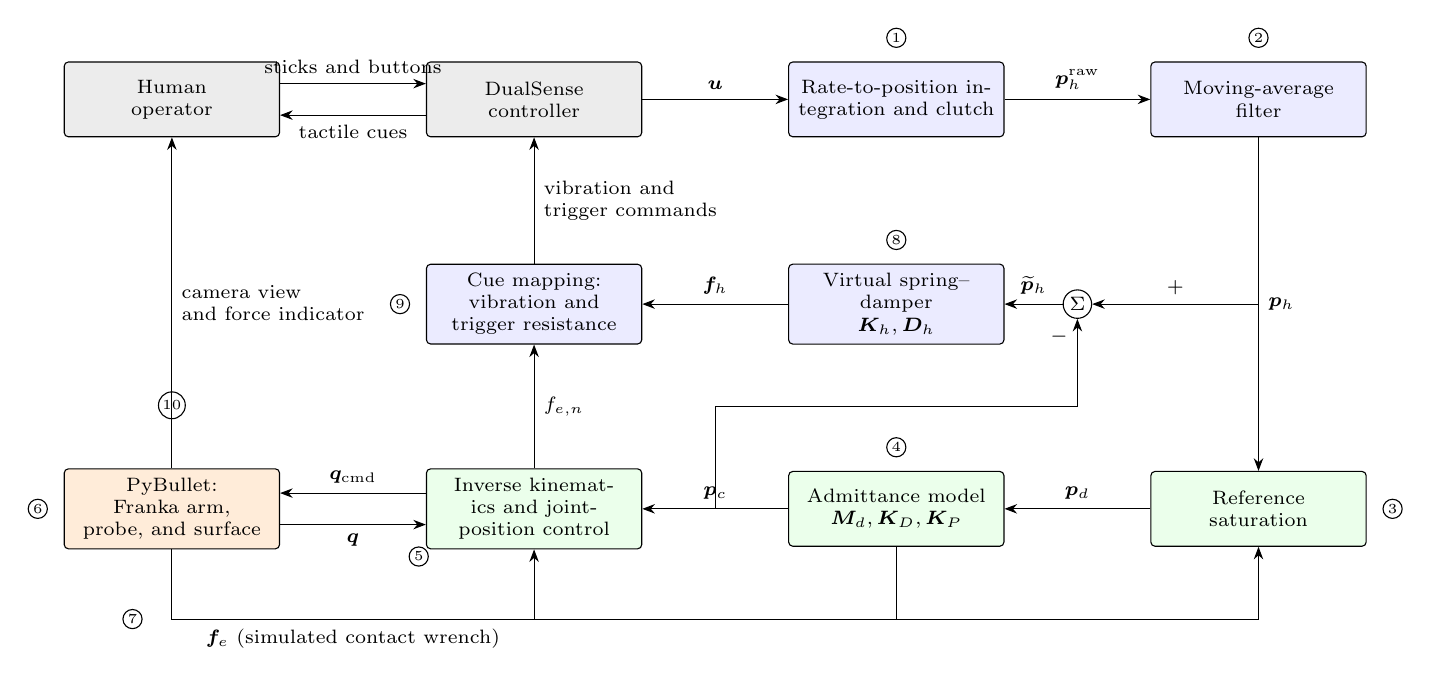
\begin{tikzpicture}[
  font=\scriptsize, >={Stealth[length=1.6mm]},
  blk/.style={draw,rounded corners=1.5pt,minimum width=2.7cm,minimum height=0.95cm,align=center,text width=2.5cm},
  op/.style={blk,fill=gray!15},
  hc/.style={blk,fill=blue!8},
  rc/.style={blk,fill=green!8},
  sm/.style={blk,fill=orange!15},
  num/.style={circle,draw,inner sep=0.8pt,font=\tiny}]
\node[op] (hum) at (0,0) {Human\\operator};
\node[op] (ds) at (4.6,0) {DualSense\\controller};
\node[hc] (int) at (9.2,0) {Rate-to-position integration and clutch};
\node[hc] (ma) at (13.8,0) {Moving-average\\filter};
\node[hc] (cue) at (4.6,-2.6) {Cue mapping: vibration and trigger resistance};
\node[hc] (vsd) at (9.2,-2.6) {Virtual spring--damper\\$\K_h,\D_h$};
\node[circle,draw,inner sep=1pt] (sum) at (11.5,-2.6) {$\Sigma$};
\node[sm] (pb) at (0,-5.2) {PyBullet:\\Franka arm, probe, and surface};
\node[rc] (ik) at (4.6,-5.2) {Inverse kinematics and joint-position control};
\node[rc] (adm) at (9.2,-5.2) {Admittance model\\$\M_d,\K_D,\K_P$};
\node[rc] (sat) at (13.8,-5.2) {Reference\\saturation};
\draw[->] ($(hum.east)+(0,.2)$) -- node[above]{sticks and buttons} ($(ds.west)+(0,.2)$);
\draw[->] ($(ds.west)+(0,-.2)$) -- node[below]{tactile cues} ($(hum.east)+(0,-.2)$);
\draw[->] (ds) -- node[above]{$\bm{u}$} (int);
\draw[->] (int) -- node[above]{$\p_h^{\mathrm{raw}}$} (ma);
\draw[->] (ma) -- node[right]{$\p_h$} (sat);
\draw[->] (sat) -- node[above]{$\p_d$} (adm);
\draw[->] (adm) -- node[above]{$\p_c$} (ik);
\draw[->] ($(ik.west)+(0,.2)$) -- node[above]{$\bm{q}_{\mathrm{cmd}}$} ($(pb.east)+(0,.2)$);
\draw[->] ($(pb.east)+(0,-.2)$) -- node[below]{$\bm{q}$} ($(ik.west)+(0,-.2)$);
% virtualized feedback: p_h (+) and p_c (-) into the summing junction
\draw[->] (13.8,-2.6) -- node[above,pos=.5]{$+$} (sum.east);
\draw[->] (6.9,-5.2) -- (6.9,-3.9) -| node[pos=.9,left]{$-$} (sum.south);
\draw[->] (sum) -- node[above]{$\pt_h$} (vsd);
\draw[->] (vsd) -- node[above]{$\f_h$} (cue);
\draw[->] (cue.north) -- node[right,pos=.5,align=left]{vibration and\\trigger commands} (ds.south);
% contact wrench returns
\coordinate (bus) at (0,-6.6);
\draw (pb.south) -- (bus) -| (adm.south);
\draw[->] (bus -| sat.south) -- (sat.south);
\draw (bus -| sat.south) -- (bus);
\draw[->] ($(bus -| ik.south)$) -- (ik.south);
\draw[->] (ik.north) -- node[right,pos=.5]{$f_{e,n}$} (cue.south);
\node[below] at (2.3,-6.6) {$\f_e$ (simulated contact wrench)};
\draw[->] (pb.north) -- node[right,pos=.5,align=left]{camera view\\and force indicator} (hum.south);
% numbers
\node[num] at ($(int.north)+(0,.3)$) {1};
\node[num] at ($(ma.north)+(0,.3)$) {2};
\node[num,right=2mm of sat] {3};
\node[num] at ($(adm.north)+(0,.3)$) {4};
\node[num,below left=0mm of ik.south west] {5};
\node[num,left=2mm of pb] {6};
\node[num] at (-0.5,-6.6) {7};
\node[num] at ($(vsd.north)+(0,.3)$) {8};
\node[num,left=2mm of cue] {9};
\node[num] at ($(pb.north)+(0,.8)$) {10};
\end{tikzpicture}

\vspace{4pt}
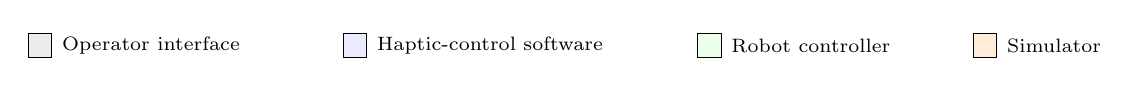
\begin{tikzpicture}[font=\scriptsize]
\node[draw,fill=gray!15,minimum size=3mm,label=right:Operator interface] at (0,0) {};
\node[draw,fill=blue!8,minimum size=3mm,label=right:Haptic-control software] at (4,0) {};
\node[draw,fill=green!8,minimum size=3mm,label=right:Robot controller] at (8.5,0) {};
\node[draw,fill=orange!15,minimum size=3mm,label=right:Simulator] at (12,0) {};
\end{tikzpicture}
\caption{Planned bilateral teleoperation architecture. The forward path converts DualSense inputs into a compliant Franka command. Return paths send the contact wrench to the admittance, saturation, and trigger channels; virtualized feedback to the vibration channel; and the camera view to the operator.}
\label{fig:block}
\end{figure*}

\begin{table*}[!t]
\caption{Annotations for the Control Architecture in Fig.~\ref{fig:block}.}
\label{tab:annot}
\centering\small
\begin{tabularx}{\textwidth}{@{}r X@{}}
\toprule
No. & Annotation\\
\midrule
1 & DualSense stick input $\bm{u}$ is scaled and integrated to form a virtual master position. This replaces the paper's 1:1 stylus mapping in (1) and (2). A controller button provides clutch and reset functions.\\
2 & The moving-average filter in (3) smooths the generated reference. Its output $\p_h$ represents the operator's unsaturated motion command.\\
3 & Reference saturation follows (10). The controller passes $\p_h$ while the normal contact force remains below $f_{th}$. Once the threshold is reached, the normal reference is held at the value defined by (11). This block is disabled in Scenarios A and B.\\
4 & The Cartesian admittance model in (5) uses $\f_d=\bm{0}$ to generate the compliant command $\p_c$.\\
5 & Inverse kinematics converts the compliant Cartesian command into Franka joint-position commands $\bm{q}_{\mathrm{cmd}}$. Joint-state feedback $\bm{q}$ is obtained from PyBullet.\\
6 & PyBullet simulates the Franka arm, inspection probe, rigid surface, robot state, probe--surface contact, and visual scene.\\
7 & The simulated contact wrench $\f_e$ is reconstructed from the probe--surface contacts, filtered, and transformed into the selected control frame.\\
8 & The virtual spring--damper in (12) generates $\f_h$ from the unsaturated error $\p_h-\p_c$. In Scenario A, the vibration channel instead uses the measured normal force.\\
9 & The DualSense provides tactile sensory substitution according to (16). The virtualized force determines vibration intensity, while the measured normal contact force determines adaptive-trigger resistance.\\
10 & A fixed PyBullet camera provides the same visual feedback in every experimental condition. A force indicator may be displayed when visual force information is part of the evaluated condition.\\
\bottomrule
\end{tabularx}
\end{table*}

\section{Literature Review}
To place the selected method in context, we reviewed research from four areas that influence our project. These include stability in bilateral teleoperation, haptic interfaces and sensory substitution, teleoperated surface-treatment systems, and force-control methods for surfaces with uncertain geometry. Table~\ref{tab:lit} compares the primary paper with the ten supporting studies and highlights how each study contributes to our proposed system.

\subsection{Bilateral Teleoperation and Stability}
Hokayem and Spong \cite{hokayem} identify stability, transparency, communication delay, and master--slave scaling as central challenges in bilateral teleoperation. Nu\~no et al.\ \cite{nuno} explain how passivity can maintain stable energy exchange among the human operator, master device, slave robot, and remote environment. These studies provide the theoretical context for the selected paper, which improves feedback behavior but does not provide a formal stability analysis.

Santiago et al.\ \cite{santiago} propose a variable $P{+}d{+}f$ controller for delayed bilateral teleoperation. Their method adjusts damping using communication delay and a feedback-power signal. Although delay compensation is outside the initial reproduction, this work provides a suitable reference for a future network-delay extension.

\subsection{Haptic Interfaces and Sensory Substitution}
Bong et al.\ \cite{bong} develop a three-degree-of-freedom motorized haptic interface using virtual spring--damper feedback. Their system demonstrates a complete bilateral position-and-force loop, but its main contribution depends on custom force-reflecting hardware that is unavailable in this project.

Motamedi et al.\ \cite{motamedi} compare visual, vibrotactile, and pressure feedback during robotic grasp, contact, and slip-detection tasks. Although their manipulation task differs from surface inspection, the study supports tactile sensory substitution and comparative user-study conditions when true Cartesian force reflection is unavailable.

\subsection{Teleoperated Surface Treatment}
Girb\'es-Juan et al.\ \cite{girbes1} study haptic and visual assistance for dual-arm teleoperation in surface-conditioning tasks. Their evaluation includes contact behavior, completion time, and surface coverage, making it the closest application-level reference for our project. However, direct reproduction would require a dual-arm platform.

Their expanded study \cite{girbes2} combines haptic feedback, visual assistance, and inertial motion capture for remote control of a dual-arm robot. The reported surface-conditioning experiments support our selection of task time, path coverage, accuracy, and operator workload as evaluation measures.

Gonz\'alez et al.\ \cite{gonzalez} combine augmented virtuality, haptic feedback, perception, and tool-orientation assistance for industrial surface treatment. The study demonstrates the value of combining human adaptability with robot-side assistance, but its perception and visualization system is broader than the scope of this project.

\subsection{Force Control for the Surface Extension}
Nasiri and Wang \cite{nasiri} propose a hybrid force/motion controller that estimates the surface normal online from measured force and commanded velocity while compensating for tangential friction. The method does not include bilateral teleoperation, but it provides the main technical basis for extending our experiment from a planar surface to an uncertain curved surface.

Solanes et al.\ \cite{solanes} present a cooperative surface-treatment system in which the robot maintains the desired contact pressure and tool orientation while a human guides the tangential motion. Their adaptive sliding-mode controller is more complex than the selected admittance controller, but the work supports separating normal-force regulation from tangential human commands. It also motivates force-tracking and path-following errors as evaluation metrics.

Overall, the supporting literature confirms that the selected paper offers a suitable balance between relevance and reproducibility. Its admittance controller, virtualized feedback, and reference-saturation mechanism can be implemented without custom haptic hardware. The DualSense interface is treated as sensory substitution, while online surface-normal estimation provides a distinct extension beyond the original planar experiment.

\section{Reproduction and Extension Plan}
\subsection{Repeatable Task Environment}
The Phase 3 environment will initially use a fixed rigid plane, a rounded probe, a visible tracing path, and a known normal direction. The operator will move the probe tangentially while managing contact. Reset will return the Franka to a collision-free joint configuration and place the probe at a fixed stand-off from the path start. Success requires completing the path while remaining within prescribed force and workspace limits. Failure includes excessive force, prolonged loss of contact, joint-limit violation, or timeout.

\subsection{Experimental Conditions}
\begin{enumerate}
\item \textbf{Baseline:} Direct Cartesian teleoperation with visual information only.
\item \textbf{Scenario A replication:} Admittance control with direct force-to-vibration feedback and no reference saturation.
\item \textbf{Scenario B replication:} Admittance control with virtualized motion-error feedback and no reference saturation.
\item \textbf{Scenario C/paper method:} Admittance control with virtualized feedback and reference saturation.
\item \textbf{Extension:} Scenario C on a curved surface with desired normal-force tracking and online normal estimation.
\end{enumerate}
The minimum Phase 4 claim will compare Scenarios A--C. The visual-only baseline provides a simple Phase 3 reference. The curved-surface controller is explicitly separated as an extension.

\subsection{Metrics and Hypotheses}
Objective metrics will include completion time, success rate, RMS normal-force error, peak force, time above the safety threshold, contact-loss count and duration, path error, surface coverage, command smoothness, and saturation activity. PyBullet's known geometric normal will permit direct measurement of normal-estimation error in the extension.

The main hypotheses are:
\begin{itemize}
\item \textbf{H1:} Virtualized feedback reduces high-frequency feedback variation and operator-command oscillation relative to direct force feedback.
\item \textbf{H2:} Reference saturation reduces peak force, excessive-force duration, and task failures relative to the same feedback without saturation.
\item \textbf{H3:} Haptic sensory substitution reduces force error and contact loss relative to visual-only operation without substantially increasing completion time.
\item \textbf{H4 (extension):} Online normal estimation reduces normal-force and path error on curved surfaces relative to a fixed-normal controller.
\end{itemize}

\subsection{User-Study Outline}
A within-subject design will expose each participant to the same task under counterbalanced feedback and control conditions after standardized practice. Objective logs will be combined with a short workload and usability questionnaire. The study will avoid claiming true Cartesian force reflection: participants receive tactile cues representing the paper's virtual-feedback signal.

\begin{table*}[!t]
\caption{Comparison of the Primary Paper and Ten Supporting Studies.}
\label{tab:lit}
\centering\scriptsize
\renewcommand{\arraystretch}{1.15}
\begin{tabularx}{\textwidth}{@{}p{2.3cm}p{2.5cm}p{3.6cm}p{3.6cm}X@{}}
\toprule
Work & Publisher/venue & Main contribution & Use in this project & Main limitation\\
\midrule
Pagliara et al.\ \cite{pagliara} & IEEE CASE 2024 & Admittance control, virtualized feedback, and reference saturation & Primary reproduction architecture & No formal stability proof or controlled user study; some implementation details are missing\\
Hokayem and Spong \cite{hokayem} & Elsevier Automatica, 2006 & Foundational bilateral-teleoperation survey & Stability--transparency framework & Survey rather than an implementation\\
Nu\~no et al.\ \cite{nuno} & Elsevier Automatica, 2011 & Passivity-based bilateral control & Energy and stability interpretation & Not specific to surface contact\\
Santiago et al.\ \cite{santiago} & Springer IJDC, 2024 & Delay-aware variable $P{+}d{+}f$ control & Reference for a future delay extension & Not specific to surface tasks\\
Bong et al.\ \cite{bong} & Springer Microsystem Technologies, 2022 & Powered three-DoF haptic master & Bilateral feedback and virtual-coupling reference & Requires custom master hardware\\
Motamedi et al.\ \cite{motamedi} & IEEE ICRA 2016 & Comparison of visual, vibrotactile, and pressure feedback & Sensory-substitution and user-study design & Grasp and slip task rather than surface inspection\\
Girb\'es-Juan et al.\ \cite{girbes1} & IEEE Transactions on Haptics, 2021 & Haptic and visual assistance for surface conditioning & Closest task and metrics reference & Requires a dual-arm platform\\
Girb\'es-Juan et al.\ \cite{girbes2} & Springer JMMUI, 2022 & Multimodal dual-arm surface teleoperation & Evaluation procedure and workload measures & Requires motion capture and dual-arm hardware\\
Gonz\'alez et al.\ \cite{gonzalez} & Elsevier JMS, 2021 & Augmented-virtuality surface teleoperation & Industrial task and shared-assistance reference & Large perception and visualization scope\\
Nasiri and Wang \cite{nasiri} & IEEE UR 2024 & Online surface-normal estimation and friction compensation & Curved-surface extension & No human interface or haptic return path\\
Solanes et al.\ \cite{solanes} & Elsevier ISA Transactions, 2018 & Human-guided surface treatment with automatic force control & Normal-force regulation and surface metrics & Two force sensors and complex sliding-mode control\\
\bottomrule
\end{tabularx}
\end{table*}

\begin{thebibliography}{11}
\bibitem{pagliara} L. Pagliara, E. Ferrentino, A. Chiacchio, and G. Russo, ``Safe haptic teleoperations of admittance controlled robots with virtualization of the force feedback,'' in \emph{2024 IEEE 20th Int. Conf. Automation Science and Engineering (CASE)}, 2024, pp. 1574--1579.
\bibitem{hokayem} P. F. Hokayem and M. W. Spong, ``Bilateral teleoperation: An historical survey,'' \emph{Automatica}, vol. 42, no. 12, pp. 2035--2057, 2006.
\bibitem{nuno} E. Nu\~no, L. Basa\~nez, and R. Ortega, ``Passivity-based control for bilateral teleoperation: A tutorial,'' \emph{Automatica}, vol. 47, no. 3, pp. 485--495, 2011.
\bibitem{santiago} D. D. Santiago, E. Slawi\~nski, L. R. Salinas, and V. A. Mut, ``Force and position coordination for delayed bilateral teleoperation of a manipulator robot,'' \emph{Int. J. Dynamics and Control}, vol. 12, pp. 1679--1693, 2024.
\bibitem{bong} J. H. Bong, S. Choi, J. Hong, and S. Park, ``Force feedback haptic interface for bilateral teleoperation of robot manipulation,'' \emph{Microsystem Technologies}, vol. 28, pp. 2381--2392, 2022.
\bibitem{motamedi} M. R. Motamedi, J.-B. Chossat, J.-P. Roberge, and V. Duchaine, ``Haptic feedback for improved robotic arm control during simple grasp, slippage, and contact detection tasks,'' in \emph{2016 IEEE Int. Conf. Robotics and Automation (ICRA)}, 2016, pp. 4894--4900.
\bibitem{girbes1} V. Girb\'es-Juan, V. Schettino, Y. Demiris, and J. Tornero, ``Haptic and visual feedback assistance for dual-arm robot teleoperation in surface conditioning tasks,'' \emph{IEEE Trans. Haptics}, vol. 14, no. 1, pp. 44--56, 2021.
\bibitem{girbes2} V. Girb\'es-Juan, V. Schettino, L. Gracia, J. E. Solanes, Y. Demiris, and J. Tornero, ``Combining haptics and inertial motion capture to enhance remote control of a dual-arm robot,'' \emph{J. Multimodal User Interfaces}, vol. 16, pp. 219--238, 2022.
\bibitem{gonzalez} C. Gonz\'alez, J. E. Solanes, A. Mu\~noz, L. Gracia, V. Girb\'es-Juan, and J. Tornero, ``Advanced teleoperation and control system for industrial robots based on augmented virtuality and haptic feedback,'' \emph{J. Manufacturing Systems}, vol. 59, pp. 283--298, 2021.
\bibitem{nasiri} E. Nasiri and L. Wang, ``Hybrid force motion control with estimated surface normal for manufacturing applications,'' in \emph{2024 21st Int. Conf. Ubiquitous Robots (UR)}, 2024, pp. 125--132.
\bibitem{solanes} J. E. Solanes, L. Gracia, P. Mu\~noz-Benavent, J. V. Miro, V. Girb\'es, and J. Tornero, ``Human--robot cooperation for robust surface treatment using non-conventional sliding mode control,'' \emph{ISA Trans.}, vol. 80, pp. 528--541, 2018.
\end{thebibliography}
\end{document}
